\documentclass[12pt,a4paper]{report}
\usepackage[utf8x]{inputenc}
\usepackage{graphicx}
\usepackage[labelfont=bf]{caption}
\usepackage{float}
\usepackage{hyperref}
\usepackage{amsmath}
\usepackage[export]{adjustbox}
\usepackage{color}
\usepackage{xcolor}

\usepackage{wrapfig}
\usepackage{lscape}
\usepackage{rotating}

\usepackage{tikz}
\usetikzlibrary{automata,positioning,arrows}

\usepackage{listings}
\lstset{basicstyle=\footnotesize, numbers=left, captionpos=b, frame=bt, linewidth=\textwidth, numberstyle=\tiny, showstringspaces=false}

\colorlet{punct}{red!60!black}
\definecolor{background}{HTML}{EEEEEE}
\definecolor{delim}{RGB}{20,105,176}
\colorlet{numb}{magenta!60!black}

\lstdefinelanguage{json}{
    basicstyle=\normalfont\ttfamily,
    numbers=left,
    numberstyle=\scriptsize,
    stepnumber=1,
    numbersep=8pt,
    showstringspaces=false,
    breaklines=true,
    frame=lines,
    backgroundcolor=\color{background},
    literate=
     *{0}{{{\color{numb}0}}}{1}
      {1}{{{\color{numb}1}}}{1}
      {2}{{{\color{numb}2}}}{1}
      {3}{{{\color{numb}3}}}{1}
      {4}{{{\color{numb}4}}}{1}
      {5}{{{\color{numb}5}}}{1}
      {6}{{{\color{numb}6}}}{1}
      {7}{{{\color{numb}7}}}{1}
      {8}{{{\color{numb}8}}}{1}
      {9}{{{\color{numb}9}}}{1}
      {:}{{{\color{punct}{:}}}}{1}
      {,}{{{\color{punct}{,}}}}{1}
      {\{}{{{\color{delim}{\{}}}}{1}
      {\}}{{{\color{delim}{\}}}}}{1}
      {[}{{{\color{delim}{[}}}}{1}
      {]}{{{\color{delim}{]}}}}{1},
}

% Windows
\graphicspath{{C:/Users/achantreau/Documents/GitHub/BEng-Individual-Project/Report/images/}}
\newcommand{\listings}{C:/Users/achantreau/Documents/GitHub/BEng-Individual-Project/Report/listings/}

% Linux
%\graphicspath{{/homes/ac6609/Documents/BEng-Individual-Project/Report/images/}}
%\newcommand{\listings}{/homes/ac6609/Documents/BEng-Individual-Project/Report/listings/}

\usepackage{fancyhdr}
\setlength{\headheight}{30pt}
\pagestyle{fancy}

\renewcommand{\chaptermark}[1]{\markboth{#1}{}}
\renewcommand{\sectionmark}[1]{\markright{#1}{}}

\fancyhf{}
\lhead{\fancyplain{}{\thepage}}
\chead{}
\rhead{\fancyplain{}{\textit{\leftmark}}}
\rfoot{\thepage}

\setlength\parindent{0pt}
\setcounter{page}{1}
\pagenumbering{roman}

\newcommand{\HRule}{\rule{\linewidth}{0.5mm}}
\newcommand{\me}{\mathrm{e}}

\begin{document}

%-----------------------------------------------------------
% TITLE SECTION
%-----------------------------------------------------------
\begin{titlepage}
\begin{center}

\textsc{\LARGE Imperial College London}\\[1.5cm]

\textsc{\Large BEng Individual Project - Final Report}\\[0.5cm]

% Title
\HRule \\[0.4cm]
{ \huge \bfseries jSCAPE - Java Self-assessment Center of Adaptive Programming Exercises \\[0.4cm] }

\HRule \\[1.5cm]

% Author and supervisor
\begin{minipage}{0.4\textwidth}
\begin{flushleft} \large
\emph{Author:}\\
Alexis \textsc{Chantreau}
\end{flushleft}
\end{minipage}
\begin{minipage}{0.4\textwidth}
\begin{flushright} \large
\emph{Supervisor:} \\
Dr.~Tristan \textsc{Allwood}
\end{flushright}
\end{minipage}

\vfill

% Bottom of the page
{\large \today}

\end{center}
\end{titlepage}

%-----------------------------------------------------------
% ABSTRACT SECTION
%-----------------------------------------------------------
\begin{abstract}
Programming is generally acknowledged to be a difficult discipline to learn, requiring problem solving skills, attention to detail and the ability to think abstractly. Yet, there is a definite interest in this subject as demonstrated by the number of students enrolling in computer science courses. \newline

In these courses, it is usually difficult for teachers and students to get an idea of how they are performing as they can only rely on a few assignments. This project aims to address this issue, by providing a solution which increases the amount of practise and feedback available to students and teachers.\newline

The result is a complete product in the form of jSCAPE (Java Self-assessment Center of Adaptive Programming Exercises) with core features consisting of providing programming exercises, displaying performance statistics, adapting the difficulty of exercises and generating exercises automatically.\newline

We used a difficulty category based algorithm, as well as concepts presented in Item Response Theory to adapt the difficulty of exercises to the student's ability.
\end{abstract}

%-----------------------------------------------------------
% ACKNOWLEDGEMENTS SECTION
%-----------------------------------------------------------
\renewcommand{\abstractname}{Acknowledgements}
\begin{abstract}
I would like to thank Dr. Tristan Allwood for proposing this project as well as providing guidance and support throughout. I would also like to thank my personal tutor, Prof. Duncan Gillies, for overseeing my time at Imperial. Last, but not least, I would like to thank my family, especially my parents for supporting me and always being there for me.
\end{abstract}

%-----------------------------------------------------------
% TABLE OF CONTENTS SECTION
%-----------------------------------------------------------
\tableofcontents

\newpage
\setcounter{page}{1}
\pagenumbering{arabic}

%-----------------------------------------------------------
% LIST OF FIGURES SECTION
%-----------------------------------------------------------
\listoffigures

%-----------------------------------------------------------
% LIST OF LISTINGS SECTION
%-----------------------------------------------------------
\renewcommand*{\lstlistlistingname}{List of Code Listings}
\lstlistoflistings

%-----------------------------------------------------------
% INTRODUCTION SECTION
%-----------------------------------------------------------
\chapter{Introduction}

\section{Motivation}
Programming is generally acknowledged to be a difficult discipline to learn, requiring problem solving skills, attention to detail and the ability to think abstractly. One could say that these skills are somewhat developed in high school during mathematics courses, but programming is still a ``beast" of its own. In addition, different programming paradigms exist, such as functional programming or imperative programming. Knowing how to program in Java can still make learning Haskell a difficult process.\newline

Yet, in this 21st century society, programming is definitely a useful skill to have, and there is an interest in the population to learn these skills. Indeed, this can be seen by the number of students enrolling in computer science courses at universities, or the increase in websites such as Codecademy\cite{Codecademy}, Coursera\cite{Coursera}, Udacity\cite{Udacity}, which provide online computer science/programming courses for free.\newline

In many of these situations, it is difficult for teachers, lecturers or course leaders to provide enough support through exercises, assignments and to monitor student's progress in such a way which allows them to modify their teaching to help struggling students. Indeed, teachers and students can generally only rely on a few homework assignments to get an idea of how they are doing. Coming up with a solution to increase the amount of practise and feedback would be beneficial to both students and teachers. \newline

Thus, there is a clear need to provide a platform for students to practise their programming skills and understanding of programming concepts, in a context of self-assessment only. In such a system, requiring teachers to come up with all the exercises by themselves can be both time consuming and ineffective: some exercises may not be challenging enough for certain top students, or on the contrary too difficult for struggling students, which can be discouraging for them.

\section{Objectives}
Having identified the problems associated with teaching and learning programming, we were led to formulating objectives in order to make the project successful and useful to the parties involved. \newline

The main objective of the project was to produce a web-based application to be used in self-assessing one's programming knowledge, whether it be in high school, at university or as part of an online course. For this application, four key features were identified:

\begin{itemize}
\item \textbf{Programming questions/exercises -} The web platform should allow students to practise their programming skills and understanding of programming concepts. There should be no limit to the number of questions a student can answer, so that if a student desires more practice, then he should be able to do that. Additionally, it should be possible for a specific set of people, such as teachers, lecturers or tutors, to add questions/exercises to the system.
\item \textbf{Progress tracking -} Designated people, such as teachers, lecturers or tutors, should have access to detailed statistics about the students performances. This will provide them with useful information about difficulties particular students, or the entire class, may be facing. In addition, the system should give feedback to the students, in the form of simple statistics, allowing them to identify their weak areas and thus improve on them.
\item \textbf{Adaptive difficulty -} The questions or exercises presented to the students should be suited to their ability. Not only will this stimulate the learning process, but it will also give a better indication of a student's understanding of the programming concepts being tested.
\item \textbf{Automated generation -} There should be a mechanism to allow for some degree of automated or semi-automated generation of exercises. This will provide a large supply of ``fresh" questions, so that students don't end up answering the same questions and memorizing the answers to them.
\end{itemize}

While investigating existing solutions (chapter \ref{chap:related-work}) we found out that some of these features were less common than others. The availability of programming exercises and progress tracking are very essential in such systems, therefore many of the related software we looked at implemented these features. On the other hand, relatively few tools integrated some form of adaptive difficulty. Finally, almost none of the tools featured automated generation of questions, opting instead to allow exercises to be added manually to the system, or downloaded from existing exercise banks.

\section{Contributions}
Within the context given above, this project makes the following contributions:
\begin{itemize}
\item \textbf{jSCAPE}: a web application for students, named Java Self-assessment Center of Adaptive Programming Exercises, with the following features:
      \begin{itemize}
      \item[-] the ability to view programming exercises and answer them while receiving feedback, a so called form of self-assessment.
      \item[-] graphs, tables and pie charts displaying statistical data on the student's performance.
      \item[-] three different exercise selection algorithms, that decide which is the best exercise to present to the student.
      \end{itemize}
\item \textbf{Admin tool}: a tool for teachers/lecturers/tutors for:
      \begin{itemize}
      \item[-] displaying student performance statistics.
      \item[-] displaying exercise statistics.
      \item[-] defining exercise categories.
      \item[-] adding exercises manually.
      \item[-] generating exercises automatically.
      \end{itemize}
\end{itemize}

\section{Report Structure}
Chapter \ref{chap:background} will present the theoretical basis for this project and the concepts necessary to follow the implementation details of the system.\newline

Chapter \ref{chap:related-work} will give an overview of related work, and will mention how these influenced the design of jSCAPE, in particular which features would be useful for such as system.\newline

Chapter \ref{chap:jscape-system} will present the jSCAPE system in detail, showing all the features which are available.\newline

Chapter \ref{chap:implementation} will cover the design and implementation details of the jSCAPE system, in particular how the difficulty of exercises is adapted to the student's ability and how exercises can be automatically generated.\newline

Chapter \ref{chap:evaluation} will contain the results of evaluating jSCAPE as a whole, and its different components. \newline

Chapter \ref{chap:conclusion} summarises the achievements of the project and discusses possible extensions that can be made to the system in the future.


%-----------------------------------------------------------
% BACKGROUND SECTION
%-----------------------------------------------------------
\chapter{Background}
% Add maximum likelihood background explanation
% Add Bayesian probability background explanation
%Add note to say that we use the word examinee to mean someone taking a test although the test may not be an exam per say.

\section{Computer Based Tests}
CBT abbreviation
- offers advantages such as being able to display higher quality visuals such as pictures, videos, graphs, etc...
- low paperwork, everything is stored on the computer
- automatic grading, less work for teachers
- generation of statistics is made easier by the fact that the data can be processed by the computer
- nowadays a lot of learning is done on computer systems, and children are used to dealing with computers so assessment through this medium is advantageous. \newline

CBTs are typically "fixed-item" tests where all the students answer the same set of questions,  usually provided by the person responsible for the assessment. This isn't ideal since students can be presented with questions that are too easy or too difficult for them to answer. Consequently, the results of the test won't give a very accurate representation of a student's ability, and for this reason, these types of tests aren't extremely useful. This problem lead to research and the development of computerized adaptive testing (CAT).

\section{Computerized Adaptive Testing}
Computerized adaptive testing (CAT), also called \textit{tailored testing}, is a form of computer-based testing which administers questions (referred to as \textit{items} in the psychometrics literature) of the appropriate difficulty by adapting to the examinee's ability.
For example, if an examinee answers an item correctly, then the next item presented will higher on the difficulty scale. On the other hand, if they answer incorrectly, they will be presented with an item lower on the difficulty scale. \newline

From an architectural perspective, a computerized adaptive test (CAT) consists of five components \cite{CAT-Framework}:

\subsubsection{1. Calibrated item pool}
An item pool is needed to store all the items available for inclusion in a test. This item pool must be calibrated with a psychometric model. During this phase, the item parameters are estimated according to the chosen model and scaled to fit with already existing items. Usually, the psychometric model employed in these systems is called Item Response Theory (IRT) (section \ref{subsec:IRT}). Calibration is a complex process, and to be done accurately it requires a considerable amount of data. Typically, it is performed by psychometricians, aided by expensive and sophisticated calibration software.

\subsubsection{2. Starting point}
Initially, when zero items have been administered, no information is known about the examinees and so the CAT is unable to estimate their ability. As a result, the item selection algorithm will fail to choose the next item to be administered.
If there is previous information available, for example an examinee's ability estimate in a closely related subject, then this can be input into the system to form the starting point configuration. Often this data isn't available or too costly to collect, so the CAT's initial ability estimate for the examinee corresponds to the mean on the ability scale - hence the first item presented will be of average difficulty.

\subsubsection{3. Item selection algorithm}
The item selection algorithm chooses the next item to present to the examinee based on the ability estimate of the examinee up to that point. Several methods exist and largely depend on the psychometric model in use. One of the most commonly used methods is the \textit{maximum information method} (section \ref{subsec:IRT}), which selects the item which maximizes the information function with respect to the estimated ability at that point.

\subsubsection{4. Scoring algorithm}
The scoring algorithm refers to the steps taken to update the examinee's ability estimate after an item has been answered. The two most commonly used methods are \textit{maximum likelihood estimation} (SECTION REFERENCE) and \textit{Bayesian estimation} (SECTION REFERENCE).

\subsubsection{5. Termination criterion}
The termination criterion specifies when the CAT should finish. For example the CAT can terminate when the change in the ability estimate after each iteration is below a certain threshold, or when time has run out, or when $N$ items have been administered, etc... Obviously, the CAT shouldn't be terminated too early, so as to allow enough time to estimate the examinee's ability with acceptable accuracy.

\begin{figure}[H]
\centering
\includegraphics[scale=1]{cat_flowchart}
\caption{Flowchart of an adaptive test. Adapted from \cite{SIETTE}.}
\label{fig:cat_flowchart}
\end{figure}

The flowchart in figure~\ref{fig:cat_flowchart} corresponds to components 2-5, and illustrates the basics of the algorithm implemented in CAT. \cite{CAT-Wiki} gives a more detailed description of the procedure:
\begin{itemize}
\item[1.] The pool of items that haven't been administered yet is searched to determine the best item to present to the examinee, according to the current estimation of his ability.
\item[2.] The chosen item is presented to the examinee, who then answers it correctly or incorrectly.
\item[3.] The ability estimate is updated, based upon this new piece of information and the previous ability estimate.
\item[4.] Steps 1–3 are repeated until a termination criterion is met.
\item[5.] The algorithm returns a final ability estimate for the examinee's performance along with a confidence level: a percentage value indicating how accurate the estimate is.
\end{itemize}

CATs offer several advantages over traditional CBTs. As a result CATs have been used in many areas\cite{CAT-Areas}, such as education, job hiring, counselling, clinical studies, etc... Since CATs administer items by adapting to the examinee's ability, the test-taking experience ends up being a more positive one. Indeed, examinees won't have to deal with answering items which are too difficult or too easy compared to their ability level, a problem which appears in traditional CBTs.\newline

In addition, by administering only those items which will yield additional information, CATs end up being more accurate in estimating an examinee's ability level. This contrasts with CBTs which usually provide the best precision for examinees of medium ability, whereas extreme scores end up being less accurate.\newline

Lastly, CATs can come up with an ability estimate much quicker and with fewer administered items when compared to traditional CBTs. Indeed, an adaptive test can typically be shortened by 50\% and still maintain a higher level of precision than a fixed version.\cite{Weiss1984}
\newline

Despite the advantages mentioned above, CATs have some limitations. A frequent complaint is that an examinee isn't allowed to go back and change his answer to a past item. This limitation exists to prevent the examinee from intentionally answering items incorrectly to make subsequent items easier, and then going back and selecting the correct answers to achieve a perfect score. For similar reasons, it isn't possible to skip items, the examinee must select an answer to move on to the next item.\newline

The second issue has to do with the items themselves. First of all, there is the need for a large bank of items to cater to all ability levels. Developing an item pool of sufficient size can be very time consuming. David J. Weiss writes in \cite{Weiss1985} that item pools with 150-200 items are to be preferred.

Secondly, for the CAT to be of good quality the item pool needs to be calibrated accurately. This requires pre-administering the items to a sizeable sample and then simultaneously estimating all the item parameters for each item. The guidelines in \cite{CAT-Primer} suggest that sample sizes may be as large as $1000$ examinees. This phase is costly, time consuming and often times simply unfeasible.\newline

Lastly, item exposure is a possible security concern. Sometimes particular items may be presented too often and become overused. This may result in examinees becoming familiar with them and sharing them to other examinees of the same ability level, thus corrupting the results of the test. This problem can be solved to some extent by modifying the item selection algorithm to include some exposure control mechanism.\newline

A brief overview of CATs was given in this section. All of these concepts will be explored in more detail in item response theory (section \ref{subsec:IRT}) and in the implementation of adaptive testing in jSCAPE (chapter XX?).

\section{Probabilistic Test Theory}
Blablablakskdjfksdjfksdsdfk stuff about probability and their usage

\subsection{Maximum Likelihood}
% Add maximum likelihood background explanation
% Conditional probability quick overview?
% Add Bayesian probability background explanation
% Bayesian networks
% Latent variables ?

IRT is based on the idea that the probability of a correct/keyed response to an item is a mathematical function of person and item parameters. 

\begin{itemize}
\item Calculates the probability of a particular student answering a specific item correctly.
\item Different IRT models: One-Parameter Logistic (1-PL), Two-Parameter Logistic (2-PL), Three-Parameter Logistic (3-PL). Refers to the number of parameters used in the model. Parameters are: 

\begin{itemize}
\item[-] item difficulty parameter (\textit{b})
\item[-] item discrimination parameter (\textit{a})
\item[-] chance/guessing parameter (\textit{c})
\end{itemize}

\item Item Characteristic Curve, i.e. probability distribution
\end{itemize}

\subsection{Bayes probability theory}

\subsection{Item Response Theory}
\label{subsec:IRT}
For these reasons, Item response theory (IRT) has seen frequent usage when it comes to CATs....We present the different models developed to predict the probability of a correct or incorrect response to a particular item.
\subsubsection{The one-parameter logistic model}
dfsdfsdf
\subsubsection{The two-parameter logistic model}
dfsdfsdf
\subsubsection{The three-parameter logistic model}
dfsdfsdf


%-----------------------------------------------------------
% RELATED WORK SECTION
%-----------------------------------------------------------
\chapter{Related Work}
%Add some context information and introduction before delving into the related work.

Web-based/Computer based education and adaptive web-based assessment systems are a ``hot" research area, and as a result, numerous tools, environments and infrastructures have emerged. There are common features to all, however some distinguish themselves by having not so common features.
Automated exercise generation in these tools is usually non-existent or very limited. Moreover, the tools are more focused on assessing students rather than self-assessment, i.e. students take tests which count towards their final grade on these systems.\newline

There are many components involved in this project, two of the more important ones are adaptive difficulty and automated generation of exercises, so there are many tools which exist which do one or the other, very rarely both.\newline

In this section we look at related software and evaluate them with respect to the objectives listed at the beginning of the development of jSCAPE.

\section{Environment for Learning to Program}
Environment for Learning to Program (ELP) is an interactive web based environment for teaching programming to first year Information Technology students at Queensland University of Technology (QUT).

\section{CourseMarker}
CourseMarker is a re-design of Ceilidh, a computer based assessment system used at the University of Nottingham for 13 years. Ceilidh was quite a complete system, providing coursework, the management of modules and the presentation of module content.

\section{Automatic Exercise Generator with Tagged Documents based on the Intelligence of Students}
The Automatic Exercise Generator with Tagged Documents based on the Intelligence of Students (AEGIS)

\section{Programming Adaptive Testing}
\begin{figure}[H]
\centering
\includegraphics[width=\textwidth,height=\textheight,keepaspectratio]{PAT_adaptive_sequence}
\caption{Adaptive sequence of questions in PAT. (Source:??)}
\label{fig:PAT_adaptive_sequence}
\end{figure}

\section{Adaptive Self-Assessment Master}
Adaptive Self-Assessment Master (ASAM) is an extension to CourseMarker, which improves upon it by administering questions which are suited to the student's ability.

\section{System of Intelligent Evaluation Using Tests for Tele-education}
The System of Intelligent Evaluation Using Tests for Tele-education (SIETTE) is a web based environment for generating and constructing adaptive tests.

\section{Summary}
We have looked at some of the relevant work in the field of computer based education and assessment. We saw that SIETTE provided many of the features we set out to replicate in jSCAPE, therefore particular parts of our implementation will be inspired by SIETTE.

%-----------------------------------------------------------
% JSCAPE SYSTEM SECTION
%-----------------------------------------------------------
\chapter{The jSCAPE System}

The jSCAPE system is designed for two distinct groups of users: students and teachers/lecturers. This separation of roles lead to the development of the main application for students, and an administrator tool for teachers/lecturers.

\begin{figure}[H]
\centering
\includegraphics[width=\textwidth,height=\textheight,keepaspectratio]{jscape_use_case}
\caption{Use case diagram of the jSCAPE system.}
\label{fig:jscape_use_case}
\end{figure}

Figure \ref{fig:jscape_use_case} shows some of the main capabilities of the jSCAPE system. Students can practice their understanding of programming concepts by answering exercises provided by the lecturers, and receive feedback while doing so. In addition, students can track their progress by viewing various graphs and charts of their performance on particular exercise categories. Finally, students can access lecture notes and website links provided by the teacher. \newline

Teachers can manage the exercise bank, whether it be adding exercises manually or automatically generating new ones based on templates. They can keep track of their students' progress and thereby identify any difficulties particular students are having. Finally, teachers are responsible for adding lecture material, website links and creating student profiles to store in the database.\newline

In the rest of this chapter we take a closer look at the current available features of jSCAPE.\newline

At the time of writing this report, we would like to note that the screen shots of the application do not represent the final version of jSCAPE, in particular, the graphics and logos haven't been finalized.

\section{Student view}

\subsection{Login screen}
\begin{figure}[H]
\centering
\includegraphics[scale=0.45]{login_screen}
\caption{The jSCAPE login screen.}
\label{fig:login_screen}
\end{figure}

For a student to use jSCAPE, they need to be in possession of login credentials, usually acquired by asking the appropriate teacher or lecturer. A connection to the jSCAPE system will be rejected if the entered login details are incorrect. Otherwise, the student can proceed to jSCAPE and access its features.

\subsection{Tracking progress through statistical data}
\label{subsec:tracking-progress}
After a successful login the student lands on the Profile tab which presents information about the student, as well as statistical data on the student's performance and usage of the system.

\begin{figure}[H]
\centering
\includegraphics[width=\textwidth,height=\textheight,keepaspectratio]{profile_screen_overview}
\caption{An overview of the Profile tab in jSCAPE.}
\label{fig:profile_screen_overview}
\end{figure}

Figure \ref{fig:profile_screen_overview} shows the Profile tab after the student has logged in to the system. Profile information for the student is listed on the left hand side, in the light-blue rectangle. This information includes the student's first name, last name, user name, which class the student is in, the last time the student logged in, and the last time the student answered an exercise. \newline

The main part of the Profile tab is split horizontally between statistical data in the form of pie charts and tables, and graphical data in the form of bar charts. \newline

Figure \ref{fig:pie_chart_stats1} shows the performance of the student in a particular exercise category, in this case ``Arrays". In the example, the student has gotten 60\% of array exercises correct and thus 40\% of them wrong. The student can view the performance pie chart for other exercise categories by changing the selected category in the combo box.

\begin{figure}[H]
\centering
\includegraphics[scale=0.6]{pie_chart_stats}
\caption{Pie chart statistics for exercise category.}
\label{fig:pie_chart_stats1}
\end{figure}

\begin{figure}[H]
\centering
\includegraphics[scale=0.7]{pie_chart_stats2}
\caption{Pie chart statistics for distribution of answers.}
\label{fig:pie_chart_stats2}
\end{figure}

Another type of pie chart available in jSCAPE can be seen in figure \ref{fig:pie_chart_stats2}. This pie chart shows the distribution of answers per exercise category. This is a useful feature when a student is trying to get a balanced amount of practice in all exercise categories. \newline

Next, performance data is presented to the student in the performance summary table, shown in figure \ref{fig:performance_summary}. In this table, there is a row for every exercise category and a row for the total of each column. Each row contains the number of exercises answered, the number of correct answers and the number of wrong answers associated with a particular exercise category.

\begin{figure}[H]
\centering
\includegraphics[width=\textwidth,height=\textheight,keepaspectratio]{performance_summary}
\caption{Performance summary table.}
\label{fig:performance_summary}
\end{figure}

In the lower half of the Profile tab there is the possibility to view performance data in the form of stacked bar charts.

\begin{figure}[H]
\centering
\includegraphics[width=\textwidth,height=\textheight,keepaspectratio]{monthly_progress}
\caption{Graph data of monthly progress.}
\label{fig:monthly_progress}
\end{figure}

Figure \ref{fig:monthly_progress} shows the monthly progress of a student for the month of May 2014 and for the exercise category ``Binary Trees". The number of correct answers (in blue) and wrong answers (in red) are graphed for each day where the student answered exercises. The student can view his monthly progress in other exercise categories and other months by manipulating the appropriate combo boxes. This historical data goes back to the first month in which the student answered an exercise.

\begin{figure}[H]
\centering
\includegraphics[width=\textwidth,height=\textheight,keepaspectratio]{yearly_progress}
\caption{Graph data of yearly progress.}
\label{fig:yearly_progress}
\end{figure}

Figure \ref{fig:yearly_progress} shows the yearly progress of a student in 2014 for the exercise category ``Binary Trees". For each month where the student answered exercises, a stacked bar can be found containing the total number of correct answers (in blue) and the total number of wrong answers (in red) for that particular year and exercise category. The student can view his yearly progress in other exercise categories and other years by manipulating the appropriate combo boxes. This historical data goes back to the year in which the student first started answering exercises.

%show difficulty progression of exercises
\subsection{Practising programming}
Selecting the Practice tab brings the student to a window where exercise categories, defined by the teacher, are displayed. These categories exist to separate exercises so that students can focus on practising one particular concept at a time. \newline

Figure \ref{fig:practice_overview} gives an overview of the Practice tab in jSCAPE. In this case, seven exercise categories have been defined by the teacher: Arrays, Loops, Syntax, Conditionals, Binary Trees, Strings and Objects. Order is irrelevant, students simply choose what type of exercise they want to practice.

\begin{figure}[H]
\centering
\includegraphics[width=\textwidth,height=\textheight,keepaspectratio]{practice_overview}
\caption{An overview of the Practice tab in jSCAPE.}
\label{fig:practice_overview}
\end{figure}

Clicking one of the exercise categories will bring the student to a new window, with an exercise and some helpful information about the chosen exercise category.
Figures \ref{fig:practice_binary_trees} and \ref{fig:practice_conditionals} give examples of what this exercise view can look like.\newline

In the case of the binary tree exercise (figure \ref{fig:practice_binary_trees}), exercise data, in the form of a binary tree, is displayed on the left of the window. On the right side of the window is the exercise itself, in this case it asks what should be printed if the binary tree is traversed using the in-order algorithm, and gives four options to choose from. \newline

In the case of the exercise on conditionals (figure \ref{fig:practice_conditionals}), exercise data, in the form of a code fragment, is displayed on the left of the window. On the right side of the window is the exercise itself, in this case it asks the student to examine the code and to determine the final values of two variables, and provides again four options to choose from. \newline

On the far right of every exercise, there is a dark blue sidebar which displays a description of the programming concept or construct being practised, links to university or course lecture notes and some other websites on the Internet if further help is needed. An example sidebar is shown in figure \ref{fig:practice_sidebar}, in this case the sidebar for the ``Binary Trees" exercise category.
\newpage

\subsubsection{Example exercises}

\begin{figure}[H]
\centering
\includegraphics[width=\textwidth,height=\textheight,keepaspectratio]{practice_binary_trees}
\caption{The Practice tab view showing an exercise on binary trees.}
\label{fig:practice_binary_trees}
\end{figure}

\begin{figure}[H]
\centering
\includegraphics[width=\textwidth,height=\textheight,keepaspectratio]{practice_conditionals}
\caption{The Practice tab view showing an exercise on conditionals.}
\label{fig:practice_conditionals}
\end{figure}

\newpage

\begin{figure}[H]
\centering
\includegraphics[scale=0.75]{practice_sidebar}
\caption{An example sidebar in the Practice tab.}
\label{fig:practice_sidebar}
\end{figure}

% Out of all the features present in jSCAPE, the one that students will notice the most is the adaptive difficulty, thus we go through an example practising session that a student could experience, to illustrate how the system adapts itself to the student's ability.
% for more information on the difficulty progression or the exercise generation, look at chapter 5 for implementation details.

\newpage
\begin{figure}[H]
\centering
\includegraphics[width=\textwidth,height=\textheight,keepaspectratio]{binary_tree_progression}
\caption{Progression of binary tree exercises.}
\label{fig:binary_tree_progression}
\end{figure}

\begin{figure}[H]
\centering
\includegraphics[width=\textwidth,height=\textheight,keepaspectratio]{conditionals_progression}
\caption{Progression of conditionals exercises.}
\label{fig:conditionals_progression}
\end{figure}

\begin{sidewaysfigure}
\centering
\includegraphics[width=\textwidth,height=\textheight,keepaspectratio]{conditionals_progression}
\caption{Progression of conditionals exercises.}
\label{fig:conditionals_progression}
\end{sidewaysfigure}

\section{Teacher view}
The teacher's main access to the system is through the jSCAPE admin tool. Essentially it provides an interface to the database where all information about students, performance, exercise categories and exercises is stored. This tool was developed to allow teachers, not familiar with SQL, to still be able to retrieve useful data about students in a presentable way and to facilitate management of the exercise bank.

\subsection{Tracking student progress}
\begin{figure}[H]
\centering
\includegraphics[width=\textwidth,height=\textheight,keepaspectratio]{analyze_overview}
\caption{An overview of the Analyze tab in the jSCAPE admin tool.}
\label{fig:analyze_overview}
\end{figure}

The jSCAPE admin tool provides teachers with the ability to track student progress and performance over time. Figure \ref{fig:analyze_overview} gives an overview of the Analyze tab, where statistical data about selected students can be displayed. The information displayed is identical to that displayed in the jSCAPE Profile tab (section \ref{subsec:tracking-progress}). On the left hand side of the window, the light blue box contains options to filter which data is displayed in the main window. A close up of the filter options is shown in figure \ref{fig:analyze_select_student}.

\begin{figure}[H]
\centering
\includegraphics[scale=1]{analyze_select_student}
\caption{Selection possibilities in the Analyze tab.}
\label{fig:analyze_select_student}
\end{figure}

The jSCAPE system includes support for multiple classes to allow for both the separation of students and the separation of exercises available to a class. A teacher can select a class to view statistics about those students taking the class. This will update the list of students in the combo box, allowing the teacher to focus his attention on the performance of one particular student. \newline

Selecting a student will show their profile information in the light blue window, along with the date of their last login, and the date of their last exercise answered. In addition, the pie charts, performance table and progress graphs will be updated to reflect the performance of the selected student. Finally, there is an option to obtain a global view of the class' performance by selecting the ``Global view" option. 

\begin{figure}[H]
\centering
\includegraphics[width=\textwidth,height=\textheight,keepaspectratio]{global_view}
\caption{Global statistics view of a class.}
\label{fig:global_view}
\end{figure}

Figure \ref{fig:global_view} shows the table that is displayed after selecting the global view option. This table shows all the students who have answered exercises in a particular exercise category. In the example above, the data shown is for the ``Syntax" exercise category. The student user names are listed along with the number of exercises they have answered, and a detailed breakdown of the number of correct and wrong answers in terms of raw values and percentages. \newline

There is a combo box to select which exercise category to display, but this isn't shown in the picture to minimize the size of it. The global view feature is useful for teachers to identify which students may be facing difficulties. They can then select the student in the Analyze tab to get more detailed statistics and information about the student's progress.

\subsection{Managing the exercise bank}
\begin{figure}[H]
\centering
\includegraphics[width=\textwidth,height=\textheight,keepaspectratio]{exercises_admin_overview}
\caption{An overview of the exercise bank management tab.}
\label{fig:exercises_admin_overview}
\end{figure}

\subsubsection{Managing exercise categories}
add description, lecture links and helpful links

set exercise category to not visible, useful feature if the class isn't ready to answer exercises of this category because the relevant material hasn't been taught yet, but the teacher still wants to prepare the exercises in advance to save time.

\begin{figure}[H]
\centering
\includegraphics[scale=1]{add_exercise_category}
\caption{Adding a new exercise category.}
\label{fig:add_exercise_category}
\end{figure}

\subsubsection{Viewing existing exercises}
\begin{figure}[H]
\centering
\includegraphics[scale=1]{existing_exercises}
\caption{Viewing information about existing exercises.}
\label{fig:existing_exercises}
\end{figure}

\subsubsection{Adding an exercise manually}
\begin{figure}[H]
\centering
\includegraphics[width=\textwidth,height=\textheight,keepaspectratio]{add_exercise_manually}
\caption{Adding an exercise on binary trees manually.}
\label{fig:add_exercise_manually}
\end{figure}

\subsubsection{Automatically generating exercises}
runs the appropriate exercise generator and stores the exercises in the database.
\begin{figure}[H]
\centering
\includegraphics[scale=0.9]{automated_generation}
\caption{Automatically generating a number of new exercises for a specific exercise category.}
\label{fig:automated_generation}
\end{figure}



\section{Summary}
In this section we gave an overview of the components present in the jSCAPE system. 

We showed that jSCAPE performed a lot of tracking of student's performances by storing useful statistics concerning their progress. In addition\newline

In the following chapter, we talk more about the design of the system and various interesting implementation details and difficulties faced during the development of this project.



%-----------------------------------------------------------
% IMPLEMENTATION SECTION
%-----------------------------------------------------------
\chapter{Design and Implementation}
\label{chap:implementation}
Talk about design choices such as only multiple choices, no exercises asking to write code, writing custom server, etc...

Mention three tier architecture

implemented as a JavaFx applet
javafx provides useful statistics package....pie charts, graphs, tables...

list tools+technology and evaluate advantages/disadvantages

java programming exercises, binary trees and code exercises to show the capabilities of the system, that it can handle multiple types of exercises.

server implementation, message codes, objectin/out streams, serverthread, show example array payload method to transfer stuff between client and server

showing feedback immediately after the exercise....cite source, shown to be most effective way of learning

piece of code + exercise involving the behaviour of the code have been found efficient (lister 2001) as far as student's assessment on their ability to read and understand the code's semantics. (NOT MY OWN WORDS) Lister, R. (2001). Objectives and objective assessment in CS1. ACM SIGCSE Bulletin, Vol. 33, No. 1, pp. 292-296.

\begin{figure}[H]
\centering
\includegraphics[width=\textwidth,height=\textheight,keepaspectratio]{three-tier-architecture}
\caption{Three tier architecture of the jSCAPE system.}
\label{fig:three-tier-architecture}
\end{figure}


CAT development, we refer back to the five components of a CAT...what item selection algorithm we use, what scoring procedure, no termination criterion, entry point is average knowledge distribution initially and attempts at a calibrated item pool, currently with teacher providing the parameters since obtaining a high quality calibrated item pool isn't something I can do.
\newpage

\lstinputlisting[caption={Item information algorithm.}]{\listings/item_information.java}

\newpage

\lstinputlisting[caption={Item response function algorithm.}]{\listings/item_response_function.java}

\newpage
\lstinputlisting[caption={Example exercise illustrating the XML format.}]{\listings/exercise.xml}

\begin{figure}[H]
\centering
\begin{tikzpicture}[>=stealth',shorten >=1pt,auto,node distance=3cm]
  \node[initial,state] (A1)      {$A1$};
  \node[state]         (A2) [right of=A1]  {$A2$};
  \node[state]         (A3) [right of=A2] {$A3$};
  \node[state]         (B1) [below of=A3] {$B1$};
  \node[state]         (B2) [left of=B1] {$B2$};
  \node[state]         (B3) [left of=B2] {$B3$};
  \node[state]         (C1) [below of=B3] {$C1$};
  \node[state]         (C2) [right of=C1] {$C2$};
  \node[state]         (C3) [right of=C2] {$C3$};


  \path[->] (A1)  edge [loop above] node {wrong} (A1)
             edge [bend left] node {correct} (A2)
        (A2) edge [bend left]  node {wrong} (A1)
             edge [bend left] node {correct} (A3)
        (A3) edge [bend left]  node {wrong} (A2)
             edge [bend left] node {correct} (B1)
        (B1) edge [bend left]  node {wrong} (A3)
             edge [bend left] node {correct} (B2)
        (B2) edge [bend left]  node {wrong} (B1)
             edge [bend left] node {correct} (B3)
        (B3) edge [bend left] node {wrong} (B2)
             edge [bend left] node {correct} (C1)
        (C1) edge [bend left] node {wrong} (B3)
             edge [bend left] node {correct} (C2)
        (C2) edge [bend left] node {wrong} (C1)
             edge [bend left] node {correct} (C3)
        (C3) edge [loop above] node {correct} (C3)
             edge [bend left] node {wrong} (C2);             
\end{tikzpicture}
\caption{State machine of adaptive difficulty categories.}
\label{state-machine}
\end{figure}

%-----------------------------------------------------------
% EVALUATION SECTION
%-----------------------------------------------------------
\chapter{Evaluation}
\label{chap:evaluation}
In this chapter we evaluate the strengths and weaknesses of jSCAPE and its various components and features, with respect to the objectives we set at the beginning of the project.

\section{Evaluating jSCAPE}
\subsubsection{Evaluating the graphical user interface}
When justifying our choices for technologies, we mentioned that one of the reasons for using Java applets and JavaFX was to provide a user-friendly and visually appealing user interface. Evidence\cite{Interface-study} suggests that students will prioritise a visually appealing user interface over powerful features. Therefore, we must make sure that our interface is generally well received amongst students, for jSCAPE to be actually useful.\newline

A small amount of data was gathered during an undergraduate fair on 02/06/2014, and during a meeting with student friends on 07/06/2014. In total we asked 10 students what they thought of the jSCAPE interface. The comments were mostly positive, however a few students mentioned that the interface was too large, requiring full screen at times. Two students also mentioned that we should be careful not to overload the view with information, particularly the Profile tab where all the statistics are displayed. We would need more data to identify possible improvements, if any, in the user interface. \newline

We didn't ask for feedback on the user interface of the admin tool as we feel this is less of a factor when it comes to whether teachers actually use the tool. Nonetheless, we think that the GUI of the admin tool is sufficiently user friendly for its purpose.

\subsubsection{Evaluating current jSCAPE exercises}
At the time of writing this report, we have implemented four exercise generators for the exercise categories of Binary Trees, Conditionals, Syntax and Strings. Some example exercises are shown in appendix \ref{chap:example-jscape-exercises}. \newline

For Binary Tree exercises, we supply a binary tree as exercise data, and ask the student to select what is printed after a specific traversal order. This type of exercise was intended to show that it was possible to bring variety to jSCAPE exercises. We think that this exercise is useful for learning the different traversal orders, however the exercise loses its usefulness very quickly once a student has mastered traversal orders. Perhaps this exercise would be more effective if we asked the student to type in the whole traversal instead of selecting the correct answer among the four different traversals.\newline

Next, for Conditionals and Strings exercises, we display a code snippet as exercise data, and ask the student to determine the final value of one or more variables. The usefulness of this type of exercise has been demonstrated in research. Indeed, \cite{Lister} has shown that this type of exercise provides effective assessment on a student's understanding of code semantics.\newline

Thanks to our random code generators, jSCAPE is able to provide many of such exercises, with very different code snippets. This means that a teacher could automatically generate 1000 Conditionals exercises and all of them would include very different code snippets, thus providing students with a large supply of exercises to self-assess their understanding of control flow in Java. However, sometimes the generated code can end up being too random, and the control flow doesn't resemble anything that would appear in a ``real" program. As such, more work would be needed in the code generating component, to make the generated code more useful in the learning process. \newline

Finally, Syntax exercises also present a code snippet, but this time containing syntax errors. The exercise asks the student to spot the syntax error, or to identify how many syntax errors the piece of code contains. We believe that this is a useful exercise for students to familiarise themselves with the Java language, especially in the early stages, when students are discovering programming languages for the first time. \newline

We would like to point out that teachers and educators have more knowledge of what constitutes a useful exercise in assessing students knowledge of a particular concept. These exercises were only intended to show what can be achieved in the jSCAPE system.

\subsubsection{Evaluating the jSCAPE exercise format}
The jSCAPE exercise format was sufficient for us to implement four exercise generators for multiple choice type questions. The format is quite flexible to allow for different views to be used in providing exercise data to accompany the question. The format was also designed with other exercise types in mind. For instance, if the exercise displayer were to read \textsf{FillInBlank} in the \textsf{$<$view$>$} tag of the second \textsf{$<$display$>$} tag, then it would ignore all the \textsf{$<$choice$>$} tags and simply create a text field for the student to type in his answer. \newline

However, in general we are not that satisfied with the exercise format. It isn't very elegant and we could see it posing some restrictions in the future. \newline

\begin{lstlisting}[language=xml, caption={A modified exercise format.}, label=lst:new_exercise_format]
<?xml version="1.0"?>
<exercise>
	<display>
		<view>........</view>
		<value>.......</value>
	</display>
	<display>
		<view>........</view>
		<value>.......</value>
	</display>
	<display>
		<view>........</view>
		<value>.......</value>
	</display>
</exercise>
\end{lstlisting}

We believe that it should be modified to allow for more exercise types to be added to jSCAPE. The listing in \ref{lst:new_exercise_format} shows a possible modification, which makes the exercise format more straightforward. Each possible \textsf{$<$view$>$} could have a component implemented in Java which takes as parameter the value of the \textsf{$<$value$>$} tag. This is how the \textsf{BinaryTree} and \textsf{CodeEditor} were implemented, but for some unknown reason, we didn't think about doing the same with other views such as \textsf{MultipleChoice}. This would offer a more general purpose exercise format than jSCAPE currently has at the moment.

\subsubsection{Evaluating automated exercise generation}
Exercises of the Binary Trees category were very suitable for automated generation. Indeed, generating random binary trees with a random number of nodes is something relatively easy to do, and the randomness of the binary tree doesn't impact the quality of the exercise.\newline

For exercises which display code snippets, we mentioned before that this generated code can sometimes be too random, and that ``strange" code can sometimes be produced. This can definitely impact the quality and effectiveness of the exercise. For instance, sometimes an \textsf{if} branch would contain the statement \textsf{var6=true} followed by the exact same statement on the next line. This kind of statement would never appear in a program written by a competent programmer, thus presenting this code snippet to a student could very well be counter productive. \newline

We believe that we have shown how exercise generators can be written to provide, theoretically, endless amounts of exercises. This was one of the objectives we set for the project at the beginning of development. However, it still remains that an exercise generator must be written manually for each new type of exercise. This isn't a very scalable solution, and thus we discuss some possible improvements for automated exercise generation, in the next chapter.

\subsubsection{Evaluating computerized adaptive testing in jSCAPE}
As part of adapting the difficulty of exercises to the student's ability, we implemented two exercise selection algorithms, one based on difficulty categories and another one based on Item response theory.\newline

The difficulty category idea was inspired by PAT\cite{PAT} and we improved the algorithm to include it in jSCAPE. The improvement was based on evidence\cite{Abdullah} which suggests that at most three exercises of a given difficulty are needed to remove uncertainty from assessing a student's knowledge.\newline

The algorithm performed well, thanks to the state machine implementation it is correct in that it will always choose an exercise of the appropriate difficulty category. It is less sophisticated than the Item response theory based algorithm, however it is much easier for teachers, because all they have to do is assign the exercise to one of three categories. But the fact that there are only three exercise categories means that there is less distinction between the difficulty of exercises, as opposed to IRT where we had 11 difficulty levels and the discrimination parameter which also affected perceived difficulty.\newline

Difficulty categories could also be assigned through the automated exercise generation process. To do this we used simple metrics such as binary tree size, code length or number of variables. This worked well under the assumption that Binary Tree exercises become more difficult as they grow in size or as they become unbalanced, however we aren't sure this assumption is valid. It may be valid early on when students are learning about binary trees for the first time. \newline

Exercises with code snippets were much more suitable for automatically assigning to a difficulty category because more metrics were available. For Conditionals, we used the number of \textsf{if/else} branches and the number of variables asked for. This worked quite well, however the randomness of the code would still interfere sometimes. A more sophisticated code analysis would be needed to determine the difficulty category and we discuss some improvements in the next chapter.\newline

The more sophisticated exercise selection algorithm we implemented was based on Item response theory. We managed to test the correctness of the implemented algorithm by running a simulation, whose results are included in appendix \ref{chap:irt-simulation}. It shows that the algorithm does indeed choose the most appropriate exercise according to the student's estimated knowledge level. The knowledge distribution is also updated correctly.\newline

However, this solution did present some limitations, most notably, it requires teachers to input the item parameters, that is the difficulty and discrimination parameters. Although guidelines were given for this step, the results will be a lot less accurate than what could be achieved through using calibration software and data. Still, it provides a bit more options than the difficulty category based method. \newline

We also evaluate our system in terms of the advantages and disadvantages mentioned in CAT (section \ref{sec:CAT}). Most of the complaints for CATs are for when they are used as means to assess students for a grade which counts towards their end of year total. For instance, not being able to go back and change one's answer. In a self-assessment setting, where the results don't really count towards anything, this isn't much of a problem. However, jSCAPE does present the most common weakness of CATs, in that a large bank of calibrated exercises is needed to be effective. Finally, we mentioned that exercise exposure could be an issue in CATs, but in jSCAPE we aren't concerned about this, because the system is only intended for self-assessment.

\subsubsection{Evaluating collection of statistical data}
To determine which statistics should be collected by jSCAPE, we inspired ourselves from other software, in particular video games, with statistics such as win/losses, history over time, etc...In addition, we regularly received feedback from our supervisor, Dr. Tristan Allwood, in terms of which statistics would be useful for a teacher or lecturer in monitoring students' progress. Asking more lecturers or teachers could help in determining more useful statistics that jSCAPE could record and display to students or teachers. It would be quite easy to add more statistics, however we believe that the core useful statistics have been implemented.

\section{Summary}
In this chapter we evaluated the different components that form the jSCAPE system. We showed that collection and display of statistical data was implemented quite solidly, and that the system was able to support provision of exercises very well.\newline

However, jSCAPE did present certain limitations in its exercise format, in its exercise generators and in the adaptive difficulty component. \newline

In the next chapter we conclude the project and give some possibilities of future work which could address the weaknesses of the system discussed in this section.

%-----------------------------------------------------------
% CONCLUSION SECTION
%-----------------------------------------------------------
\chapter{Conclusion}
\section{Future Work}
We have a few ideas of where to orient the project next...

The main limiting factor was time and insufficient means to collect the large amounts of data required to obtain a high quality calibrated item pool.

\begin{itemize}
\item Very flexible system so other programming languages could be offered, i.e. cSCAPE, for C and hSCAPE for Haskell. 
\item Working more extensively on the adaptive component of the system, i.e. improving the algorithm which selects questions for students based on their estimated ability.
\item Extend system to allow admins to provide their own question templates, maybe come up with a template grammar which then allows questions to be automatically generated. Or at least allow pluggable function references which will be called to generate the exercise component.
\item Add support for more question types. JavaFX is very good in that sense since it can play audio clips, video clips, show animations, the webview component has endless possibilities thanks to the inclusion of Javascript.
\item Future Work as a research project vs future work as a commercial product
\item JavaFX applications are based on the model-view-controller pattern, so a nice split can be done in the code, however I only learnt about this two weeks into the project, so all the of the GUI components are created in the code as opposed to in the FXML file.
\item add more robust security: hashing for login/password and ssl connections between the server and client, and server database, because this communication could reveal solutions to the exercises..
\end{itemize}

%-----------------------------------------------------------
% Bibliography
%-----------------------------------------------------------
\begin{thebibliography}{9}

\bibitem{SIETTE} Conejo, R., Guzmán, E., Millán, E., Trella, M., Pérez-de-la-Cruz, J. L., \& Rios, A. (2004). SIETTE: A Web-Based Tool for Adaptive Testing. \textit{International Journal of Artificial Intelligence in Education, 14}, 29-61.

\bibitem{CAT-Wiki} Computerized adaptive testing. \url{http://en.wikipedia.org/wiki/Computerized_adaptive_testing}. Accessed: \today.

\bibitem{CAT-Framework} Thompson, Nathan A., \& Weiss, David A. (2011). A Framework for the Development of Computerized Adaptive Tests. \textit{Practical Assessment, Research \& Evaluation}, 16(1).

\bibitem{CAT-Areas} IRT-Based CAT. \url{http://www.iacat.org/content/irt-based-cat}. Accessed: \today.

\bibitem{Weiss1984} Weiss, D. J., \& Kingsbury, G. G. (1984). Application of computerized adaptive testing to educational problems. \textit{Journal of Educational Measurement}, 21, 361-375

\bibitem{Weiss1985} Weiss, D.J. (1985). Adaptive Testing by Computer, \textit{Journal of Consulting and Clinical Psychology}. 1985, 53, 6, pp. 774-789.

\bibitem{CAT-Primer} Wainer, H., \& Mislevy, R.J. (2000). Item response theory, calibration, and estimation. In Wainer, H. (Ed.) Computerized Adaptive Testing: A Primer. Mahwah, NJ: Lawrence Erlbaum Associates.




\end{thebibliography}

%-----------------------------------------------------------
% APPENDICES
%-----------------------------------------------------------
\appendix
\chapter{User Manual}
The user manual is included in the Help Tab of the jSCAPE client application. It is not reproduced here to limit the number of pages of this report.

\chapter{Example jSCAPE exercises}
\label{chap:example-jscape-exercises}

\subsubsection{Binary tree exercise}
\lstinputlisting[language={xml}, tabsize=4, caption={Example exercise for the Binary Tree exercise category}]{\listings/binary_tree_exercise.xml}

\subsubsection{Strings exercise}
\lstinputlisting[language={xml}, tabsize=4, caption={Example exercise for the Strings exercise category.}]{\listings/strings_exercise.xml}

\subsubsection{Conditionals exercise}
\lstinputlisting[language={xml}, tabsize=4, caption={Example exercise for the Conditionals exercise category}]{\listings/conditionals_exercise.xml}

\end{document}